\documentclass[11pt, oneside]{article} 
\usepackage{geometry}
\geometry{letterpaper} 
\usepackage{graphicx}
	
\usepackage{amssymb}
\usepackage{amsmath}
\usepackage{parskip}
\usepackage{color}
\usepackage{hyperref}

\graphicspath{{/Users/telliott_admin/Tex/png/}}
% \begin{center} 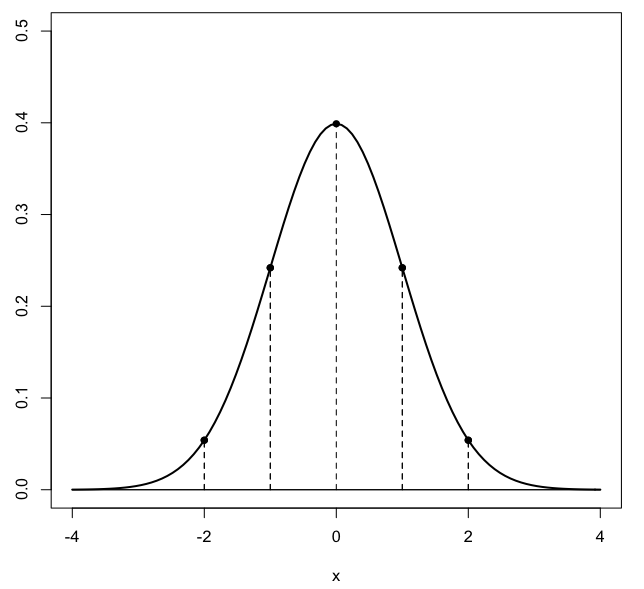
\includegraphics [scale=0.4] {gauss3.png} \end{center}

\title{Improper integrals}
\date{}

\begin{document}
\maketitle
\Large

\label{sec:Improper_integrals}

Generally speaking, an integral is improper when one of three conditions holds:  (i) the upper bound is $\lim x \rightarrow + \infty$, (ii) the lower bound is $\lim x \rightarrow - \infty$, or (iii) at one of the bounds, the value of the function is undefined $\rightarrow \pm \infty$.  

If the function's value becomes undefined in the middle of an interval, first break the integral into pieces.

Then, integrate the function anyway, and if, when we evaluate it at that problematic bound, the result is finite (often $0$), then we can use the result.

\[ \int_1^{\infty} \frac{1}{x^2} \ dx \]
\[ = - \frac{1}{x} \ \bigg |_1^{\infty}  \]
The upper bound is $\infty$, but the value of the there is zero.  So
\[ = - (- \frac{1}{1}) = 1  \]
On the other hand, the same integral with bounds $[0,1]$ blows up at the lower bound.  That area is infinite.

Here is a second example.  Compare:
\[ \int_0^1 \frac{1}{x} \ dx \]
\[ \int_0^1 \frac{1}{\sqrt{x}} \ dx \]

For both, the value of $f(x)$ becomes infinitely large (the limit does not exist) as $x \rightarrow 0$.  Nevertheless, the area under the second curve is finite, while that under the first is not.

Informally, the way we roll here is to substitute another bound, like $a$, which is very small but not zero:

\[ \int_a^1 \frac{1}{x} \ dx \]
\[ = \ln x \ \bigg |_a^1 \]
    
and now we ask, what happens if we plug in $0$ for $a$?  The value of the integral "blows up" at the lower bound.  $\ln 0$ doesn't exist and the logarithm of a very small number approaches $- \infty$.  So this integral can't be evaluated.

If we think of it as a Riemann sum with rectangles of width $1$, it is like the harmonic series (with a lower bound of $1$)

\[ 1 + \frac{1}{2} + \frac{1}{3} + \frac{1}{4} + \frac{1}{5} + \dots \]

We know this diverges.

On the other hand:
\[  \int_a^1 \frac{1}{\sqrt{x}} \ dx \]
\[ = 2 \sqrt{x} \ \bigg |_a^1 \]

Now, when we evaluate at the lower bound, with $0$ for $a$, we get $0$.  Therefore, the value of the integral is just:
\[ = 2 \sqrt{1} - 0 = 2 \]

\subsection*{negative exponential}

Here is the negative exponential function:
\[ \int_0^{\infty} e^{-x} \ dx \]
\[ = - e^{-x} \ \bigg |_0^{\infty} \]
\[ = - (0 - 1) = 1 \]

And a variation:
\[ \int_0^{\infty} 2 \pi e^{-r^2} \ r \ dr \]
Letting $t = r^2$, this is what we just did:
\[ \pi \int_0^{\infty} -e^{-t} \ dt = \pi \]

The negative exponential often appears with a constant factor, traditionally denoted by $\lambda$:
\[ \int_0^{\infty} e^{-\lambda x} \ dx \]
\[ = - \frac{1}{\lambda} \ e^{-\lambda x} \ \bigg |_0^{\infty} \]
\[ = -\frac{1}{\lambda} \ (0 - 1) = \frac{1}{\lambda} \]

This form of the negative exponential $e^{-\lambda x}$ is a valid (and famous) probability density function if the total value of the integral is equal to $1$.  We achieve this by "normalizing" it, multiplying by $\lambda$:
\[ p(x) = \lambda \int e^{-\lambda x} \ dx \]
We'll see all of these again.

\subsection*{log 1/x}

The inverse log function provides a fun example of an improper integral with a very simple and finite result.  The example (and the figure) are from Hamming.
\begin{center} 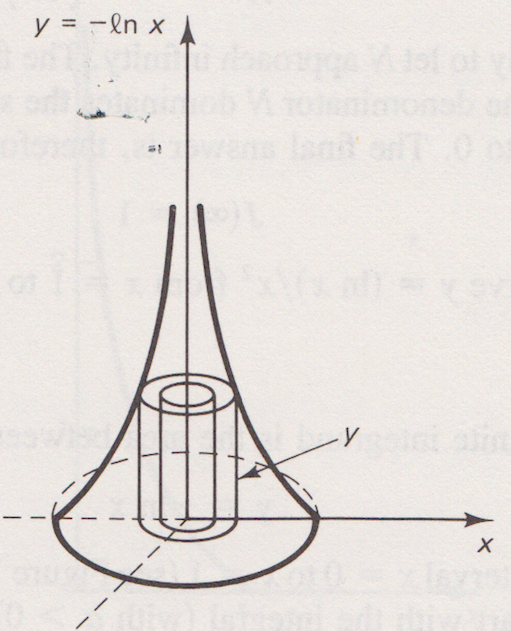
\includegraphics [scale=0.4] {log4.png} \end{center}

We consider the function
\[ y = - \ln x = \ln \frac{1}{x} \]

The minus sign is used so we are working with positive $y$, recognizing that the function is not defined at $x=0$.  Rotate the curve around the $y$ axis and find the volume.

To use the method of cylinders, we consider a series of concentric cylindrical surfaces of width $dx$, ranging from $x=0$ to $x=1$.  For each value of $x$, the surface area is the height of the function $h = - \ln x$ times the circumference $2 \pi x$ to give a volume for each element of

\[  dV = 2 \pi x \ y \ dx \]
    \[ = 2 \pi x \ (- \ln x) \ dx \]

We get the total volume by integrating over the interval $[0,1]$
\[ V = \int_0^1 2 \pi x \ (- \ln x) \ dx \]
\[ = - 2 \pi \int_0^1 x \ln x \ dx \]

Store the factor of $-\pi$ for second;  we will need the $2$ sooner.  What is 
\[ \int 2 x \ln x \ dx \]
    
The systematic approach is to use integration by parts, but let's just guess.  If we had $F(x) = x^2 \ln x$ then part of the derivative $f(x) = F'(x)$ would be what we want:

\[ \frac{d}{dx} x^2 \ln x = 2 x \ln x + \frac{x^2}{x} \]
\[ = 2 x \ln x + x \]
    
to cancel the extra $x$, we need another term, namely $-x^2/2$
\[ F(x) = x^2 \ln x - \frac{x^2}{2} \]
\[ F'(x) = 2 x \ln x + x - x \]
\[ = 2 x \ln x \]
So
\[ \int 2 x \ln x \ dx =  x^2 \ln x - \frac{x^2}{2} \]

The volume $V$ is equal to $- \pi$ times
\[ x^2 \ln x - \frac{x^2}{2} \bigg |_0^1 \]

At the upper limit, $\ln 1 = 0$ so this is $-1/2$, and the question becomes, what happens to $x^2 \ln x$ as $x$ approaches $0$?  We guess that $x^2$ must become small faster than $\ln x$ approaches $-\infty$.  So at the lower limit, we will get zero, and the whole thing is
\[ V = - \pi \ (-\frac{1}{2}) = \frac{\pi}{2} \]

Let's try by the method of disks and then come back to this limit.  We also have a figure for the second approach
\begin{center} 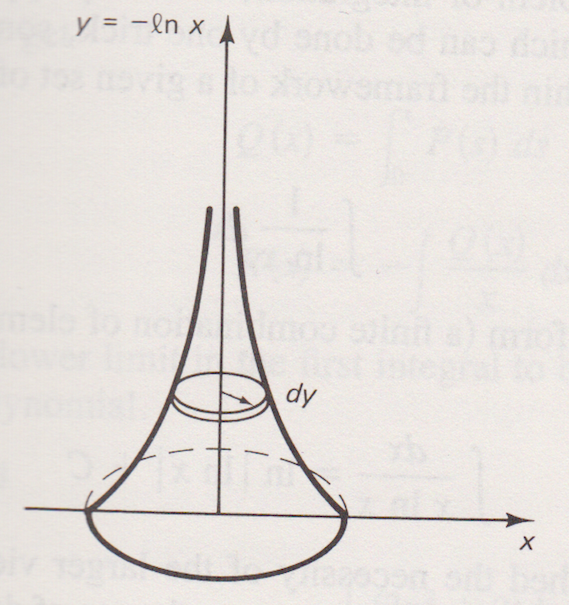
\includegraphics [scale=0.4] {log5.png} \end{center}
Again
\[ f(x) = - \ln x \]
As $y$ ranges from $0$ to $\infty$, each disk has a width $dy$ and an area equal to $\pi x^2$ so the volume element is

\[ dV = \pi x^2 \ dy \]

The next part is really interesting.  We follow Hamming.  Rather than flip the figure, we can change variables and write
\[ y = - \ln x \]
\[ dy = - \frac{1}{x} \ dx \]

so the volume element becomes
\[ = - \pi x^2 \ \frac{1}{x} \ dx \]
\[ = - \pi x \ dx \]

The limits also change.  Before we had $y = 0 \rightarrow \infty$ and now we have $x = 1 \rightarrow 0$ (because $y = - \ln x$), so
\[ V = \int_1^0 - \pi x \ dx \]
\[  = \pi \int_0^1 x \ dx \]
\[  = \frac{\pi}{2} x^2 \ \bigg |_0^1 =  \frac{\pi}{2} \]

So it looks like we were right about that limit.

But what is the formal method for evaluating
\[  \lim_{x \rightarrow 0} x^2 \ln x \]

We convert this to a fraction
\[  \lim_{x \rightarrow 0} \frac{\ln x}{1/x^{2}} \]

Since both numerator and the denominator go to $\infty$ as $x \rightarrow 0$, this is an indeterminate form, and we can use L'Hospital's rule (\hyperref[sec:Hospital]{\textbf{here}}).

We need derivatives of the numerator and the denominator.  The numerator gives $1/x$ and the denominator gives $-2/x^{3}$ so we have
\[ \frac{1}{x} \ \frac{1}{-2/x^{-3}} = \frac{x^3}{x}(- \frac{1}{2}) = - \frac{x^2}{2} \]
which in the limit as $x \rightarrow 0$, also goes to $0$.

\end{document}  